\section{Experimental Evaluation}\label{sec:evaluation}

%\subsection{Domains Setup}

%\subsubsection{Domains}

To evaluate our approach we deployed a set of domains that materialize the computational continuum --- as shown in Table~\ref{tab:domain-exp-config}. The sample application is a simplified augmented reality application, in which users can capture an image and invoke a microservice (implemented and deployed using functions within the continuum) to perform feature extraction and match them back to the image. 

For our mobile domain we used a smartphone in which we deployed the A3-E domain-side middleware and the functions needed to perform both feature extraction and matching. 

For our local-edge domains we adopted the IBM/Apache OpenWhisk serverless framework\footnote{https://openwhisk.incubator.apache.org/}. OpenWhisk is open-source, and therefore is --to date-- the only stable serverless alternative that can be deployed locally or on private clouds. 

%Particularly, openwhisk provides a built-in noSQL database: CouchDB, which is associated with the implemented actions through user-defined triggers and rules. 

We had two local-edge domains, and placed both of them in the same LAN as the origin of the requests (i.e., the client applications/devices). This was done to emulate a few-hop scenario in which devices are directly connected to their nearest edge domains. \texttt{Local-edge-1} was placed on a regular laptop, allowing us to represent a situation in which latency is close to zero, but the computational resources are highly constrained, as scaling-up is not possible due to inherent physical restrictions of the underlying infrastructure. Similarly, \texttt{local-edge-2} domain was placed on a Polimi server. In this case the computational resources are less constrained, yet low latency can still be achieved due to physical proximity.

\begin{table}[htb]
	\caption{Domains Setup in the Continuum for the Experimental Evaluation}
	\label{tab:domain-exp-config}
	\begin{tabular*}{1\textwidth}{@{\extracolsep{\fill}}>{\raggedright}p{1.5cm}>{\raggedright}p{6cm}>{\raggedright}p{6cm}}
		\toprule 
		Domain & Machine Resources & Execution Environment\tabularnewline
		\midrule
		\midrule 
		Mobile & Samsung Galaxy S6 SM-G90, 3Gb RAM, 8x Cortex CPU 2Ghz & Android 5.0.2 + Java Functions + OpenCV
		\tabularnewline
		\midrule 
		Local-edge-1  & ubuntu/trusty64-2, 4x vCPUs, 4Gb RAM & OpenWhisk, 256 Mb/Action, Python 2.7 + OpenCV \tabularnewline
		\midrule 
		Local-edge-2  & ubuntu/trusty64-2, 8x vCPUs, 16Gb RAM & OpenWhisk, 256 Mb/Action, Python 2.7 + OpenCV \tabularnewline
		\midrule 
		Cloud-FaaS & N/A & AWS Lambda, 256 Mb/Function, Python 2.7 + OpenCV \tabularnewline
		\midrule 
		Cloud-IaaS & Autos Scaling Group with t2.micro instances + Amazon Linux AMI 2017  & NodeJs 6.11 server + Python 2.7 + OpenCv
		\tabularnewline
		\bottomrule
	\end{tabular*}
\end{table}


%In this experiment, we considered two alternatives for deploying the serverless continuum architecture, mimicking the behavior of both an edge node and a fog node (Figure~\ref{fig:exp-edge}).  

%The client application is embedded in the edge node, consisting on the postman requests and the node.js endpoint (Figure~\ref{fig:exp-setup1}). 
%On the edge-local alternative, we used a virtual machine running locally, on a regular laptop, with 4x CPU, 4x Gb of RAM and 40 Gb SSD of storage. 

%For the Fog alternative, we deployed the serverless architecture on Policloud\footnote{http://policloud.polimi.it/}, the private IaaS solution of Politecnico di Milano. Here, the computational resources are less constrained, and still low latency can be achieved due to physical proximity (two hops from the client) and data locality. This setup runs on a small cluster of 4 virtual machines with 2x CPU, 4x Gb of Ram and 100 GB SSD, each running a different component of openwhisk (triggers and storage, Http server, controller, and invokers, respectively). Note that in this case the fog node is deployed in the same LAN that originates the requests, to emulate the few-hop scenario in which devices are directly connected to their corresponding MEC.

The cloud domain for this experiment used AWS Lambda\footnote{https://aws.amazon.com/lambda/}, given that it is currently the most mature serverless solution on the market. The functions and associated libraries and services (storage, feature extraction and matching) were hosted within the same AWS region. This is actually enforced by AWS to guarantee a certain degree of data locality. Finally, we also deployed the functions onto a traditional cloud domain, i.e., using cloud IaaS. 

The main goal of this experiment was not to compare traditional cloud services against a serverless solution, but to demonstrate that the proposed continuum could outperform the cloud under the tested circumstances and requirements.


\subsection{Domain Latency Evaluation} 

To compare the latency of the different domains along the continuum, we performed a first experiment in which we varied the number of clients making concurrent requests. Each client was configured to perform $100$ requests, at a constant rate of two requests per second. Each request stimulated both the feature extraction and the matching from a sample image. 

This setup was achieved taking into account the default maximum for concurrent executions in AWS Lambda\footnote{http://docs.aws.amazon.com/lambda/latest/dg/concurrent-executions.html} and Openwhisk\footnote{https://github.com/apache/incubator-openwhisk/blob/master/docs/reference.md}, as well as the limited resources of the edge domains. 

This experiment excluded the mobile domain, and focused on the remote ones, i.e., edge and cloud (see Figure~\ref{fig:exp-setup1}). Capturing and uploading an image is emulated using Postman\footnote{https://www.getpostman.com/}, a JavaScript open source application designed to load test the functional behaviors of Web APIs, and to measure their performances. The  payload for this experiment was a sample image of approximately 65 KB, which is a reasonable size for this use case considering the requirements regarding low-latency and computation time~\cite{rodriguez16mobile}. 

%Once the image was sent through HTTP/POST, the actual execution depended on the domain being used. triggering Openwhisk actions for both edge domains, AWS Lambda functions for Cloud-FaaS domain, and a Nodejs server that calls a Python function for Cloud-IaaS domain.

%was performed without using the A3-E middleware nor the device (mobile domain), since it aims to evaluate the plain latency for remote domains when processing simultaneous requests. This scenario would not occur in a mobile domain, which only process local requests. The possibility of offloading computation from one mobile device to another is left as a future work.



 

%In our edge domains for the experiment, uploading an image to CouchDB (Step 3.a) triggers the action that performs the feature extraction and matching (Step 4.a)  with the points-of-interest, supported by the OpenCV\footnote{\url{http://opencv.org}} visual recognition library (Step 5.a). 


\begin{figure}[htb]
	
	\centering
	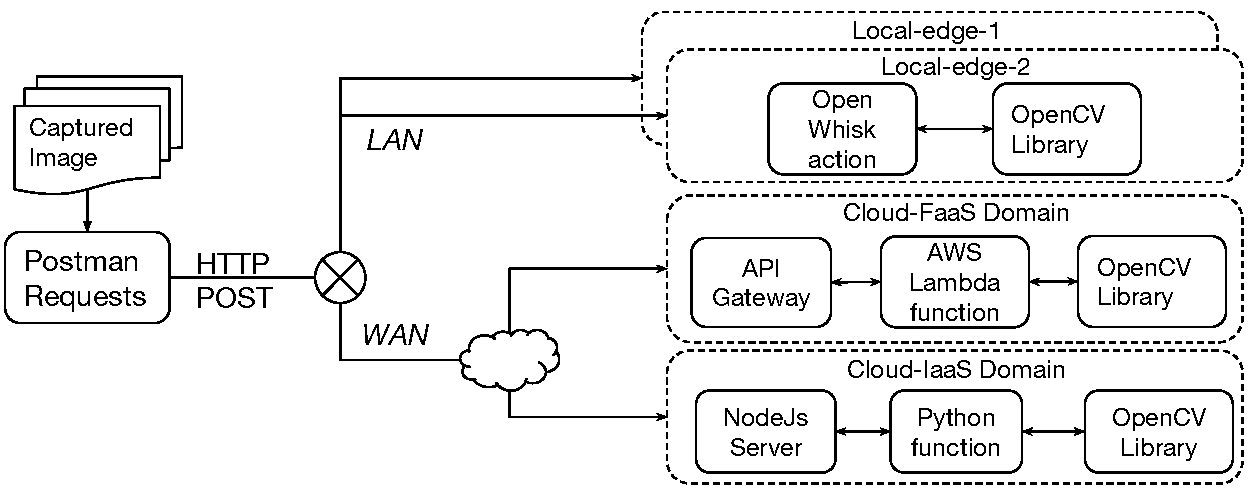
\includegraphics[width=0.95\textwidth]{figs/experimental-setup.pdf}
	\caption{Setup for Latency Experiments}
	\label{fig:exp-setup1}
\end{figure}

%\subsubsection{Baseline Latency}

 Figure~\ref{fig:latency-domains} shows the average latency for each scenario, averaged through $5$ executions. Note that the computation time (light gray) is different from the overhead (dark gray). The latter includes network communication (routing and forwarding) and queuing time (when no resources are available to process the request immediately). 

\begin{figure}
	
	\centering
	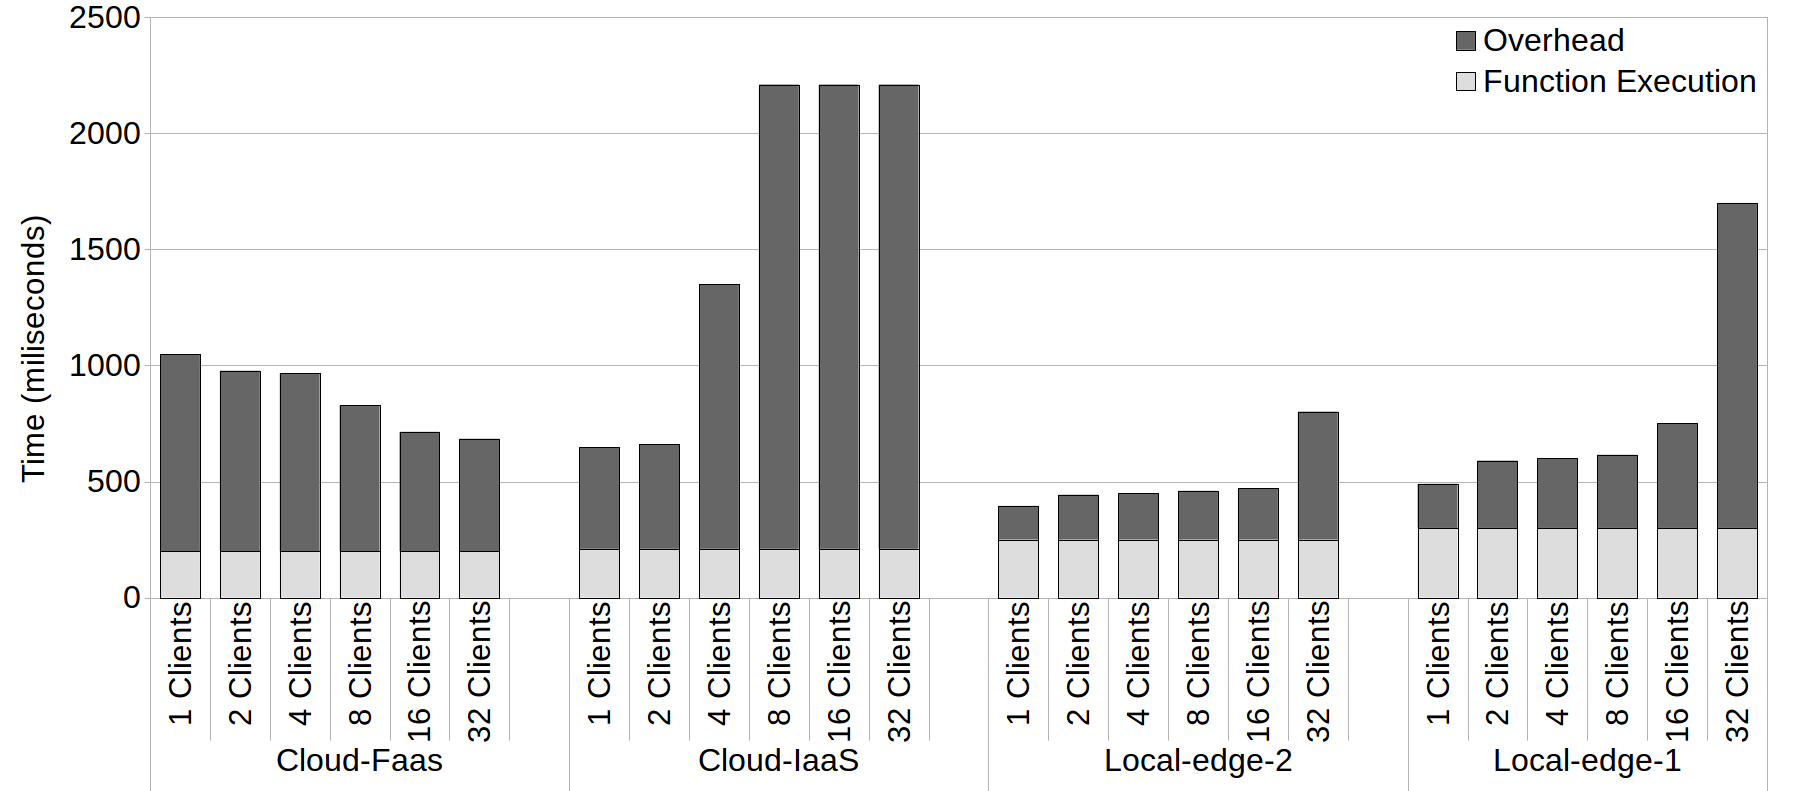
\includegraphics[width=1\textwidth]{figs/latency-domains}
	\caption{Latency results for each domain and different number of clients.}
	\label{fig:latency-domains}
\end{figure}

 When considering up to $16$ simultaneous clients, the latencies added by the edge domains are less than the latencies in both cloud alternatives. Regarding the Cloud-Faas domain, the latency reduction is up to $90$\% for \texttt{local-edge-1} and up to $82$\% for \texttt{local-edge-2} respectively. Regarding the traditional cloud domain, reductions are up to $77$\% and $58$\%, respectively. Since in Cloud-IaaS a scaling-up action (that can demand several seconds~\cite{Quatrocchi2016discrete}) triggers when more than one VM instance is needed to handle the workload, requests timeout in the meantime. 
 
 For light to medium workloads, the local-edge domains outperformed all the other alternatives. However, \texttt{local-edge-1} is the most resource-constrained, which hinders its availability under heavier workloads. Interestingly, the Cloud-IaaS domain also outperformed the serverless one ($46$\% less latency) for light workloads. This can be due to the additional steps performed by the API Gateway in order to forward RESTful calls to lambda functions in the Cloud-FaaS\footnote{http://docs.aws.amazon.com/lambda/latest/dg/with-on-demand-https.html}. Nevertheless, this advantage is mitigated by the fact that Cloud-FaaS is a serverless alternative, and as such can better react to workload bursts, thanks to its faster horizontal scaling~\cite{Villamizar2017lambda,Hendrickson:2016}.


%\subsection{Battery} The second set of experiments targeted the measurement of battery consumption of a mobile device in two scenarios: 1) in which feature extraction and matching were performed locally, and 2) these tasks were offloaded to edge servers.

\subsection{Evaluation of A3-E in the Continuum} 

In our second set of experiments we wanted to evaluate A3-E as an enabler of the computation continuum. A mobile device was setup to host the A3-E client-side middleware, which was in charge of dynamically selecting the best domain for a specific execution, based on the perceived QoS. 

Once again our sample application was the augmented reality application with feature extraction and matching provided through the continuum. In this case we had three domains: the first was the mobile domain for executing Java functions on the mobile device, the second was an edge domain implemented using OpenWhisk, while the third was an AWS Lambda cloud domain.

The experiment featured four different scenarios. The first three scenarios each considered a single different domain. The fourth scenario brought the three domains together to form the continuum. For this last scenario, we probabilistically simulated the availabilities of the three domains. 

To simulate the cases in which the mobile device was momentarily outside of the mobile network's coverage, the average unavailability of the cloud domain~\cite{garcia2017bandwidth} was set to once every $15$ minutes. A3-E was configured to ping for domain availability, as well as perceived QoS, every two seconds ($u = 2$). Using a geometric distribution\footnote{https://math.stackexchange.com/questions/165993/average-number-of-times-it-takes-for-something-to-happen-given-a-chance}, the probability of the cloud being unavailable during a ping ($internetOnToOff$) was $0.022$. Every time the cloud was unavailable, the average time for it to become available again was $2$ minutes, i.e., the probability  $internetOffToOn$ was $0.166$. 


The rationale for the edge domain is analogous, yet with a higher probability of it being unavailable --- e.g., due to the lack of physical proximity with the edge servers. In this case, the edge is unavailable once every $10$ minutes, i.e., the probability was $edgeOnToOff = 0.33$. Once unavailable, we considered that it would take an average of $5$ minutes for it to become available again, i.e. the probability $edgeOffToOn$ was $0.066$. Finally, the mobile device is always available, and therefore it was selected in our experiments when all other domains were unavailable, or the sensed latencies were too high for the application's requirements.


\begin{comment}
internetOnToOffProbability = 0.22%
internetOffToOnProbability = 1.66%

edgeOnToOffProbability = 3.33%;
edgeOffToOnProbability = 6.66%;

e = 1/p; //average number of trials it takes for the event with probability p to happen
~t = e * u;  //average time it takes for the event with probability p to happen given a trial interval u
~t = u/p; //the same, but using the trial interval and the probability p 

###

trial interval u = 2 seconds

average time for disconnecting: 15 x 60 seconds
prob. of disconnecting: 0.2222222%   

average time for reconnecting: 2 x 60 seconds
prob. of reconnecting: 1.666666%

average time for edge unavailability: 10 x 60 seconds 
prob. of edge unavailability: 0.333333%

average time for edge becoming available: 5 x 60 seconds 
prob. of edge becoming available: 0.666666%

\end{comment}

%(all-domains).

The experiment consisted in cascading 2000 sequential requests for feature extraction and matching of a sample image (with a size of 65 KB). We measured the total execution time, the battery consumption in the mobile device, and the average time per call. Figure~\ref{fig:exp-a3e} shows the experimental results, averaged among $5$ executions for each scenario.

\begin{figure}[htb]
	\raggedright
	\captionsetup[subfigure]{width=0.45\textwidth}	
	\subfloat[Total execution time (seconds)\label{fig:total-exec-a3e}] {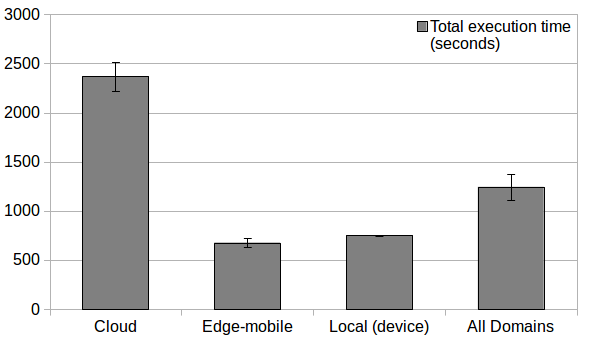
\includegraphics[width=0.45\textwidth]{figs/total-exec-time-A3E}}
	\captionsetup[subfigure]{width=0.45\textwidth}
	\subfloat[Battery consumption (\%)\label{fig:battery-a3e}] {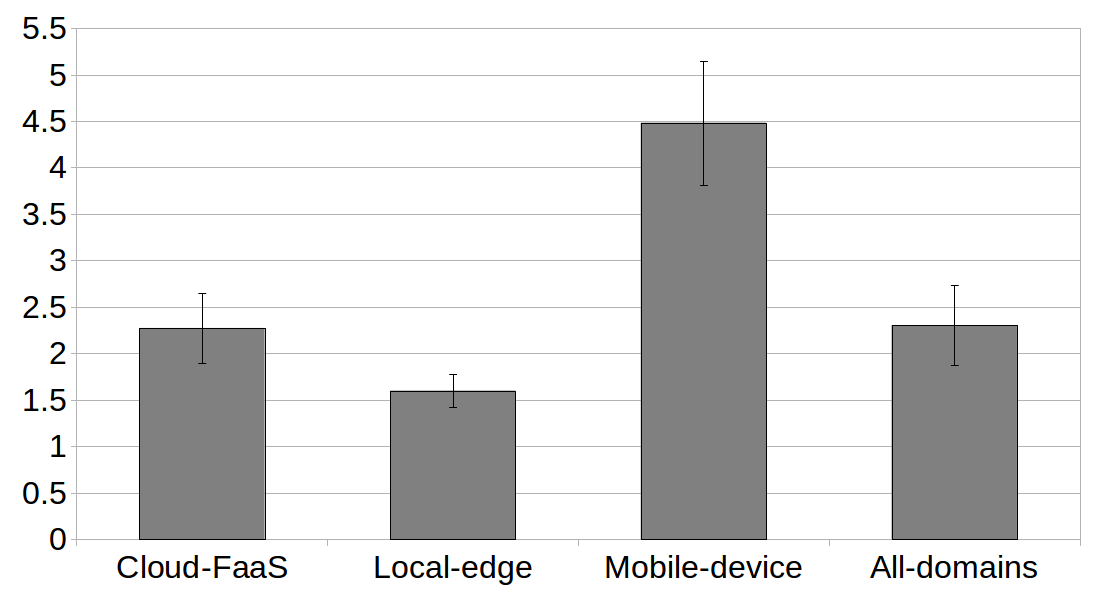
\includegraphics[width=0.45\textwidth]{figs/battery-consumption-A3E}}
	
	\captionsetup[subfigure]{width=0.45\textwidth}
	\subfloat[Execution time per call (miliseconds)\label{fig:time-per-call-a3e}] {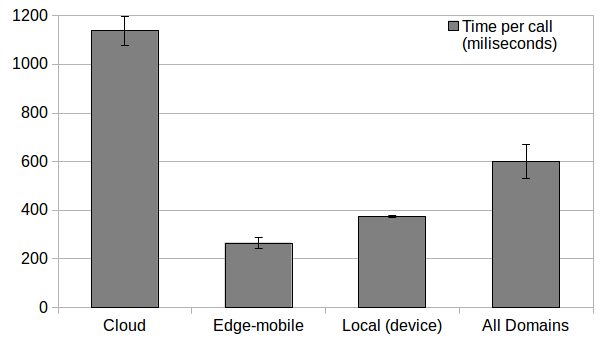
\includegraphics[width=0.45\textwidth]{figs/time-per-call-A3E}}
	\captionsetup[subfigure]{width=0.45\textwidth}
	\subfloat[Number of Calls per domain in all-domains scenario\label{fig:calls-per-domain-a3e}] {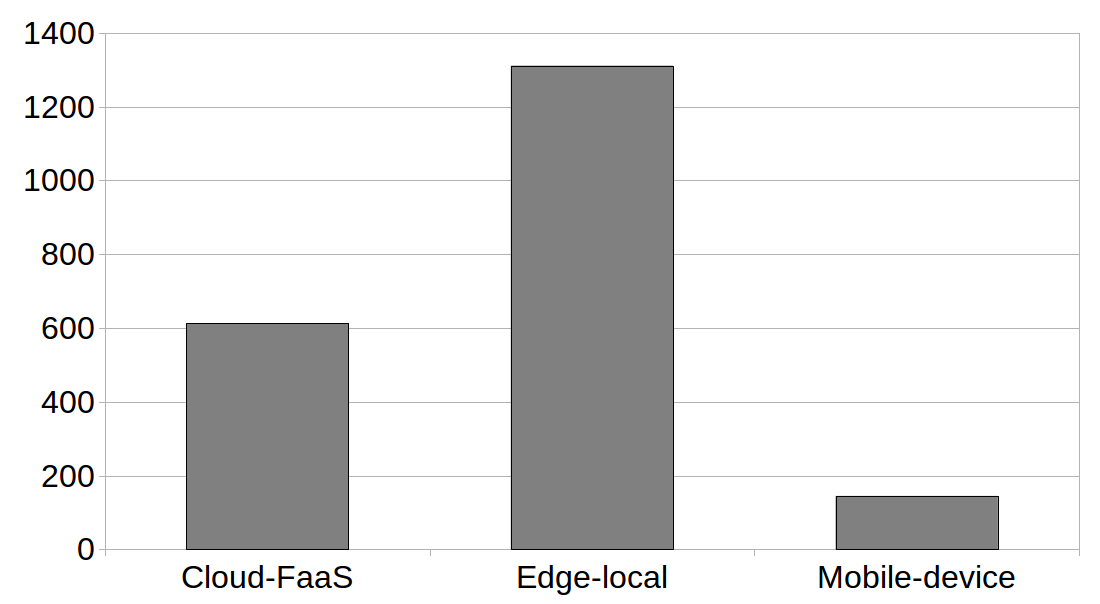
\includegraphics[width=0.45\textwidth]{figs/calls-per-domain-A3E}}
	
	\caption{A3-E experimental evaluation results} \label{fig:exp-a3e}
\end{figure}

For the total execution time (Fig.~\ref{fig:total-exec-a3e}), considering the \texttt{Cloud-FaaS} domain as a baseline, \texttt{local-edge} improved the execution time up to a $72$\%, while \texttt{mobile} and \texttt{All-domains} up to a $69$\% and $49$\%, respectively. The highest battery consumption (see Figure~\ref{fig:battery-a3e}) was when using only the \texttt{mobile} domain, with a battery drop of $4.5$\% during $750$ seconds (i.e., $12.5$ minutes) of execution. Battery savings with \texttt{Cloud-FaaS}, \texttt{local-edge} and \texttt{All-domains} were $49$\%, $35$\%, and $49$\%, respectively. The average execution time (see Figure~\ref{fig:time-per-call-a3e}), with \texttt{Cloud-FaaS} as our baseline ($1137$ milliseconds per call), was improved by $76$\%, $68$\% and $47$\% for \texttt{local-edge}, \texttt{Mobile} and \texttt{All-domains}, respectively. Finally, for the \texttt{All-domains} scenario, Figure~\ref{fig:calls-per-domain-a3e} shows the average number of calls that were processed by each domain in the continuum: $65$\% by the \texttt{local-edge} domain, followed by \texttt{Cloud-FaaS} ($30$\%) and \texttt{Mobile} ($7$\%).
 
These experiments tell us that the total execution time, when using only the cloud, was two times higher than when using the continuum (all-domains). This is because the requests were performed in cascade, and given the higher latency per call in the cloud, the total time increases accordingly. Clearly, using A3-E to switch to edge domains when possible substantially reduces the latency and improves the perceived QoS.

Battery consumption was substantially lower when offloading computation, rather than performing it on the device. The \texttt{mobile}-device scenario lasted half the time, but used twice as much battery (a prohibitive $20$\% of battery drain per hour) as the \texttt{all-domains} one, given that it was performing CPU intensive operations. This recalls the importance of computation offloading to preserve a device's resources.

Finally, the domain selection and distribution of computation performed by A3-E in the \texttt{all-domains} scenario reflects the underlying idea of the computation continuum: exploit the edge domains as much as possible (by giving them high scores in Formula~\ref{eq:smart}). This will lead to better balance among computation time and resource consumption. Switch to the cloud, or to the local device, only when necessary. Note that in this experiment the mobile-device computation was given the lowest possible score, thus the cloud was selected as the first alternative to edge domains. This behavior can be tuned by adjusting the application requirements and domain parameters discussed in Section~\ref{sec:implementation}.

%that allows to cope with unavailability and fluctuations in QoS 

%\textcolor{blue}{TODO:(2) Discuss the relevance of the results }

%\paragraph{Threats to validity}

As threats to validity is it worth mentioning that the experiments were performed targeting only one client application and, in the case of the second experiment, one client device performing requests. It is also necessary to perform simulations with multiple clients using several applications with different requirements, and the corresponding functionality deployed along the continuum. Additionally, it is currently not possible to deploy real mobile-edge domains, i.e., to provide computational capabilities on base stations. This can be approximated by deploying edge domains with different specifications in terms of computational power and latency (e.g., deploying on bare metal servers and Polimi private cloud), to better reflect the heterogeneity of the continuum. 




